\chapter{Kinematics}
\begin{center}
    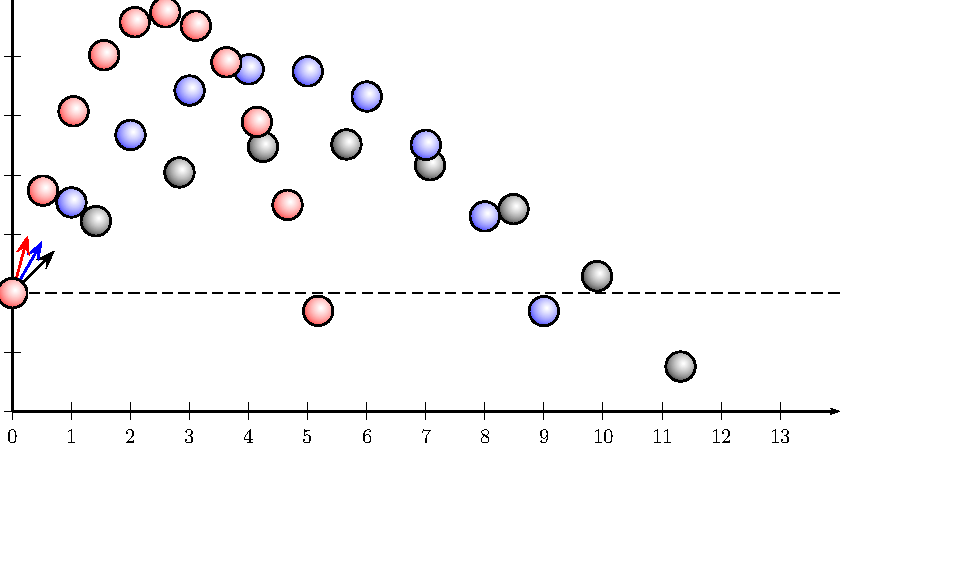
\includegraphics[width=\textwidth]{../images/Kinematics/schieferWurf.pdf}
    \captionsetup{type=figure}
    \caption[figure]{\ref{Projectile motion} Parabolic path travelled by balls thrown at varying angles.}
\end{center}
\begin{itemize}
    \item \emph{Distance} is defined as the total length of \emph{path} travelled.
    \item \emph{Displacement} is defined as the distance of a point from some reference point \emph{in a specified direction}.
    \item \emph{Velocity} is defined as the rate of change of displacement.
    \item \emph{Acceleration} is defined as the rate of change of velocity.
    \item Four key formulas for kinematics. When the  acceleration \(a\) is constant:
    \begin{enumerate}
        \item \(v=u+at\),
        \item \(s=ut+\frac{1}{2}at^2\),
        \item \(s=\frac{1}{2}(u+v)t\),
        \item \(v^2=u^2+2as\).
    \end{enumerate}
\end{itemize}